
\section{Models}

\begin{frame}[fragile]{Models}
	\begin{columns}[onlytextwidth]
		\column{.8\textwidth}
		
		\begin{figure}
			%\caption{Dog}
			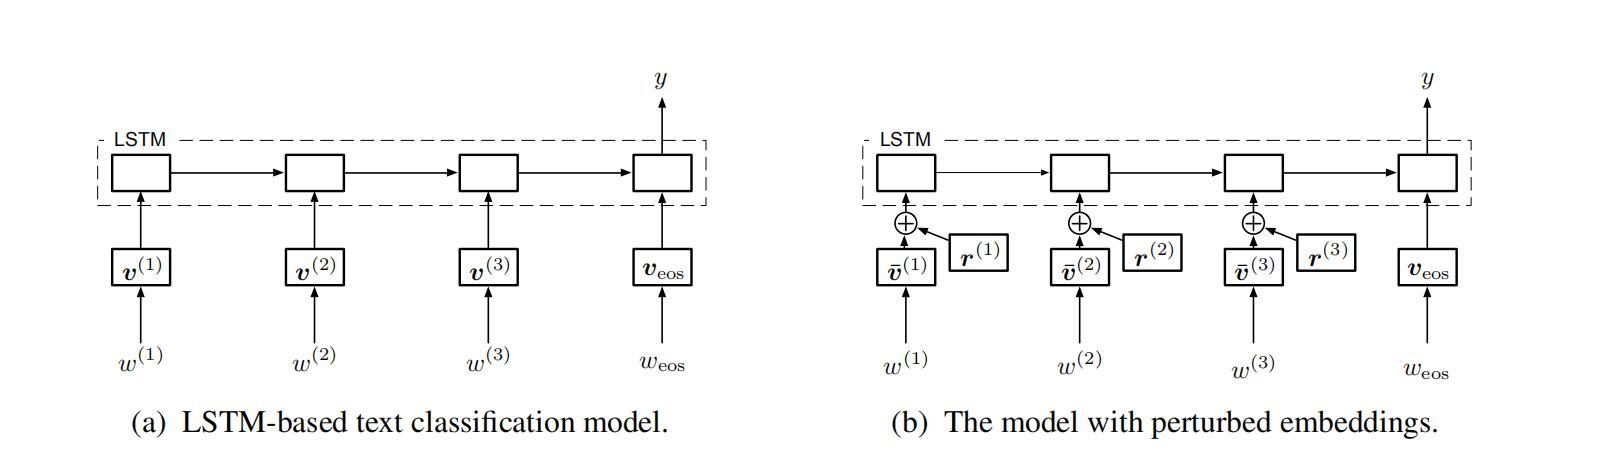
\includegraphics[height=0.5\textheight]{model.jpg}
		\end{figure}

		
	\end{columns}
	
	
\end{frame}
\section{Adversarial \& Virtual Adversarial Trianing}


\begin{frame}[fragile]{Symbols}

	\begin{table}[!htbp]
		\caption{ explanation of symbols}\label{tab:01} \centering
		\begin{tabular}{ccc}
			\toprule[1.5pt]
			symbol &  explanation of symbols\\ 
			\midrule[1pt]
			$x$ &  input vector \\
			$I$ &  input dimension \\
			$y$ &  labels \\
			$Q$ &  space of labels \\
			$p(y| x,\theta )$ & input probability distributions\\
			$D_l$ &  data with label\\
			$D_ul$ & data without label \\
			$\cdots$ & $\cdots$ \\
			\bottomrule[1.5pt]
		\end{tabular}
	\end{table}
	
\end{frame}

\begin{frame}[fragile]{Adversarial Training}
	\begin{itemize}
		\item loss function:
		\[
			L_{adv}:=D[q(y|x_l),p(y|x_l+r_{adv},\theta)] 
		\]
		\[	where\quad  r_{adv}:=arg\quad max_{r:\|r\|\leqslant \epsilon} \mathit{D}[q(y|x_l),p(y|x_l+r, \theta)]
		\]
		\item solution:
		\[
		 	r_{adv}\approx \epsilon\frac{g}{{\|g\|}^2},where \quad g=\nabla_{x_l}\mathit{D}[h(y;y_l),p(y|x_l, \theta)]
		\]
		\item or:
		\[
			r_{adv}\approx \epsilon \mathit{sign(g)}
		\]
	\end{itemize}
\end{frame}

\begin{frame}[fragile]{D? KL}
	\begin{itemize}
	\item Kullback–Leibler divergence
	\item How one probability distribution is different from a second.
	\end{itemize}

\end{frame}

\begin{frame}[fragile]{Kullback–Leibler divergence}
		\begin{columns}[onlytextwidth]
		\column{.7\textwidth}
		\begin{figure}
			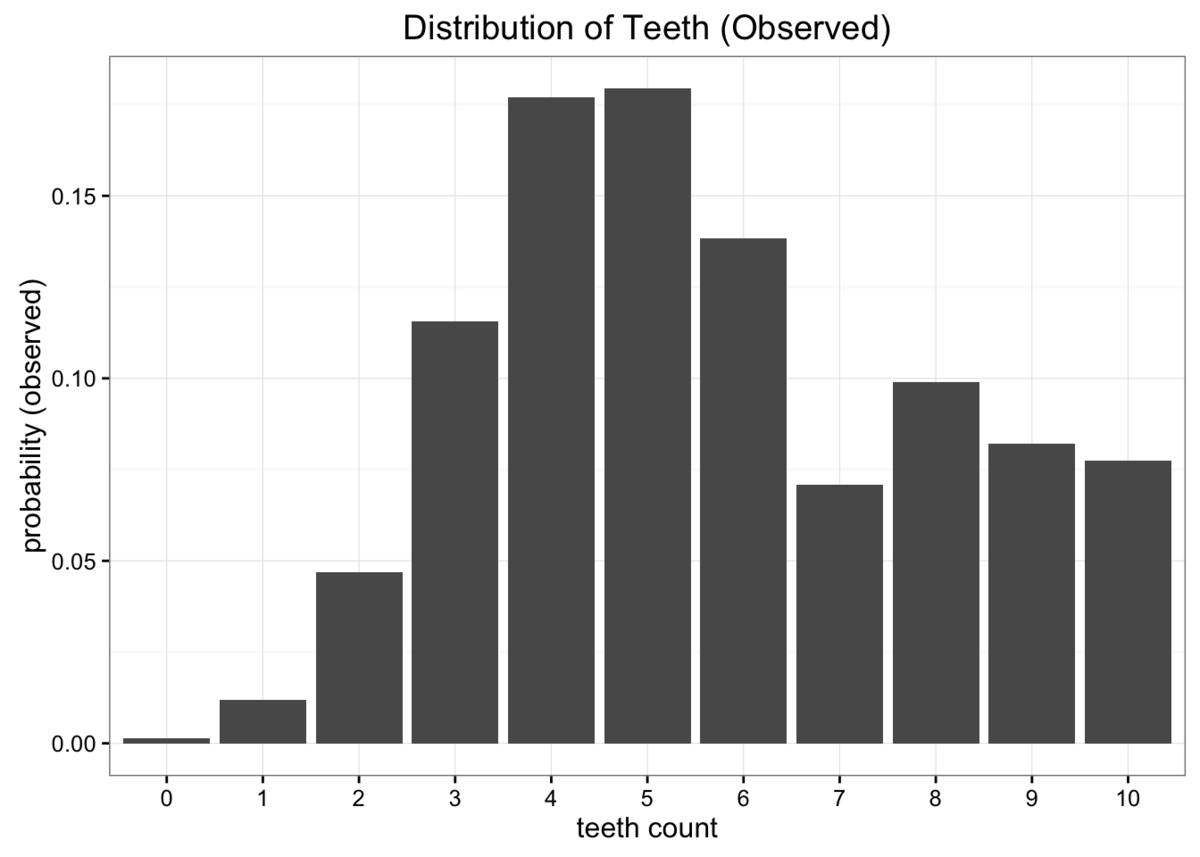
\includegraphics[height=0.8\textheight]{f1.png}
		\end{figure}
		\column{.4\textwidth}
		\begin{figure}
			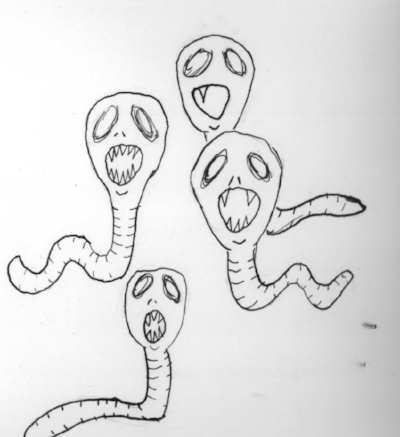
\includegraphics[height=0.5\textheight]{f2.png}
		\end{figure}

		
	\end{columns}
	
\end{frame}

\begin{frame}[fragile]{Kullback–Leibler divergence}
		\begin{columns}[onlytextwidth]
		\column{.3\textwidth}
		\begin{figure}

			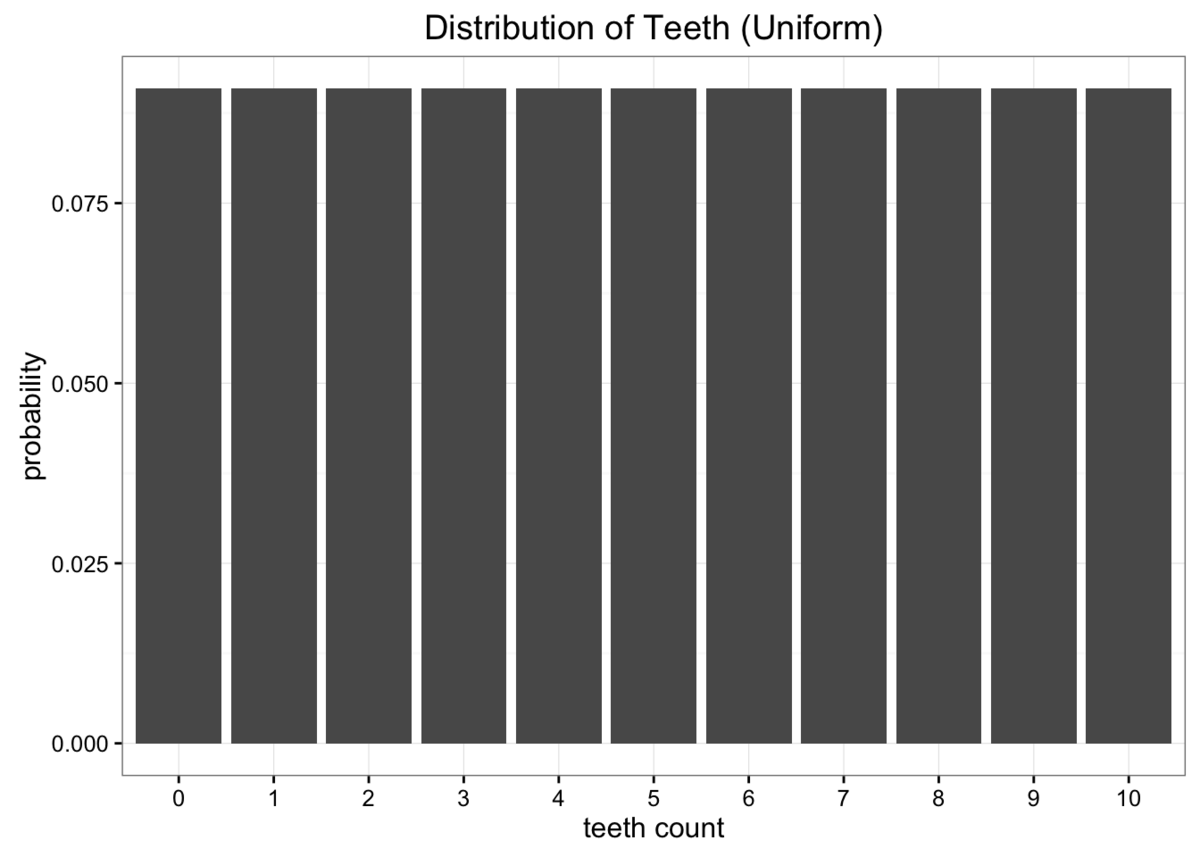
\includegraphics[height=0.5\textheight]{f3.png}
		\end{figure}
		\column{.3\textwidth}
		\begin{figure}

			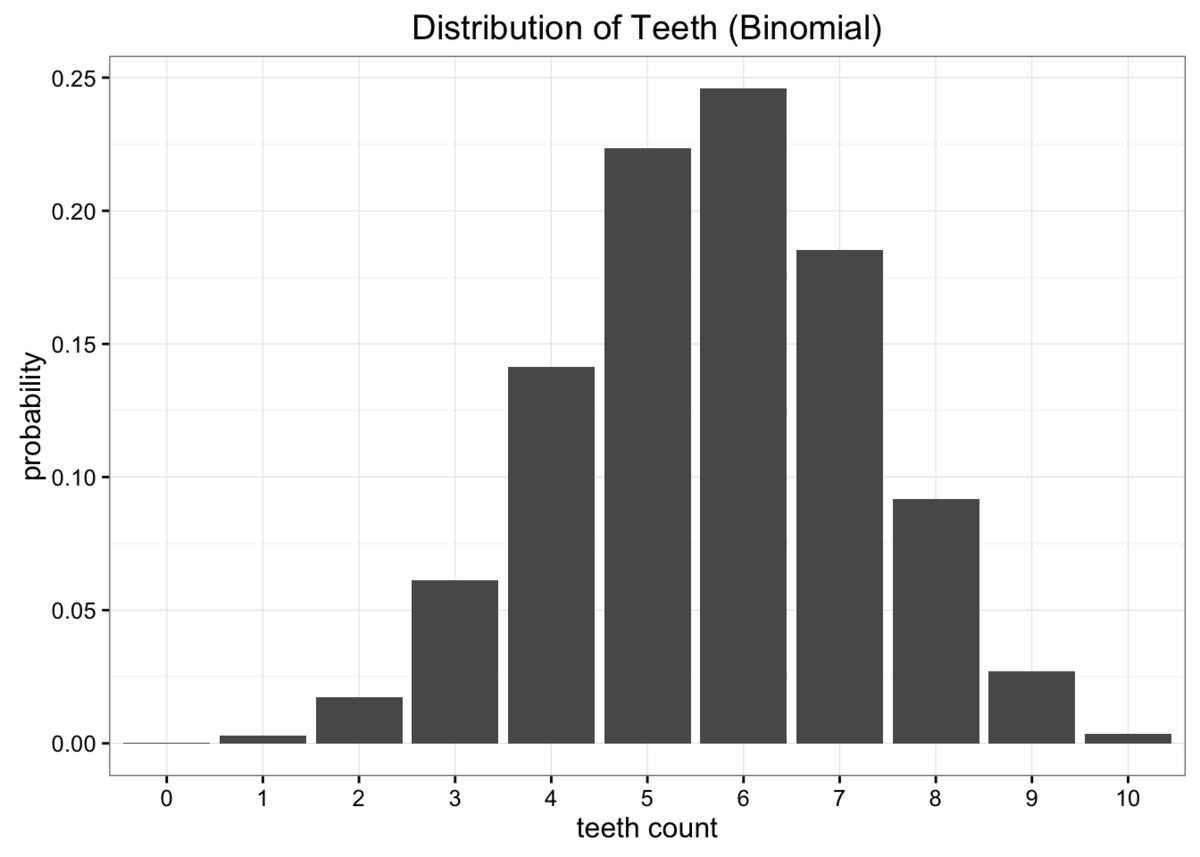
\includegraphics[height=0.5\textheight]{f4.png}
		\end{figure}
		\column{.3\textwidth}
		\begin{figure}

			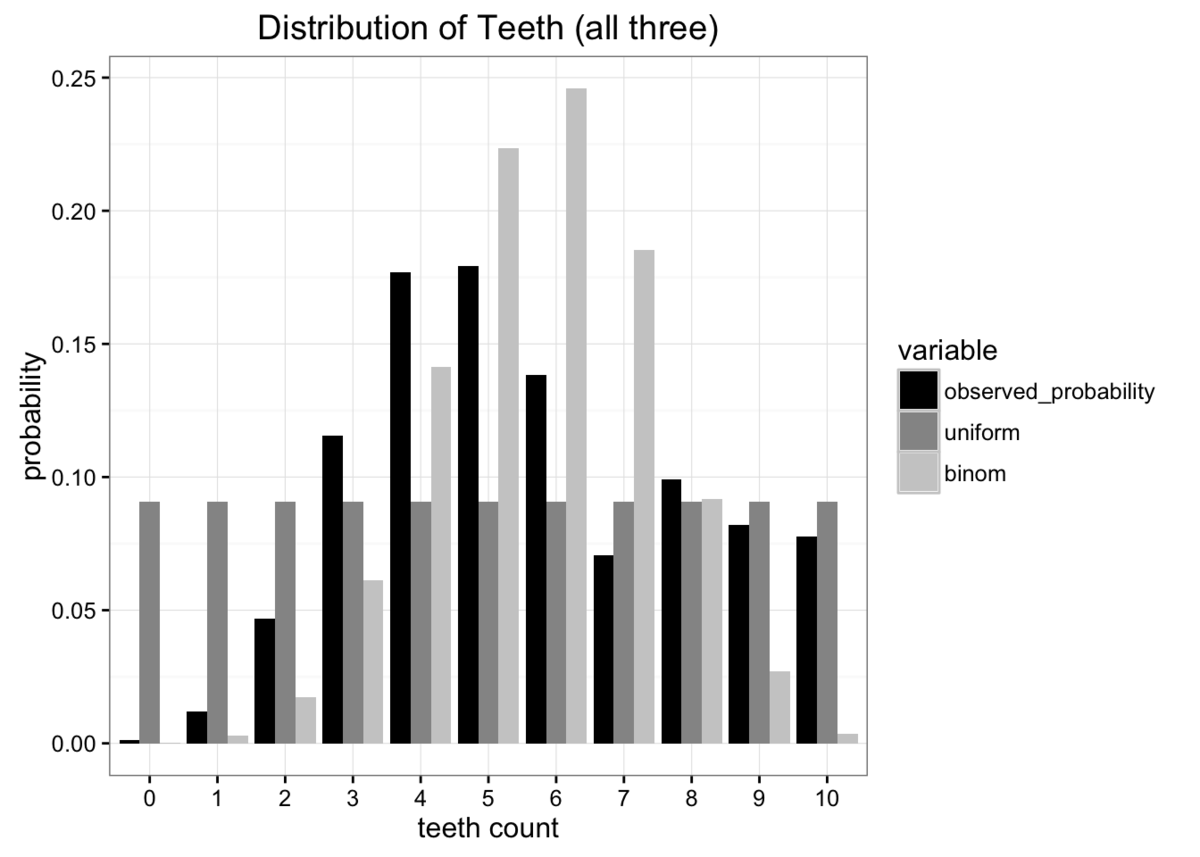
\includegraphics[height=0.5\textheight]{f5.png}
		\end{figure}
		
	\end{columns}
	
\end{frame}

\begin{frame}[fragile]{Adversarial Training}
	\begin{itemize}
		\item loss function:
		\[
		L_{adv}:=D[q(y|x_l),p(y|x_l+r_{adv},\theta)] 
		\]
		\[	where\quad  r_{adv}:=arg\quad max_{r:\|r\|\leqslant \epsilon} \mathit{D}[q(y|x_l),p(y|x_l+r, \theta)]
		\]
		\item solution:
		\[
		r_{adv}\approx \epsilon\frac{g}{{\|g\|}^2},where \quad g=\nabla_{x_l}\mathit{D}[h(y;y_l),p(y|x_l, \theta)]
		\]
		\item or:
		\[
		r_{adv}\approx \epsilon \mathit{sign(g)}
		\]
	\end{itemize}
\end{frame}

\begin{frame}[fragile]{VAT}
	\begin{itemize}
		\item target function:
		\[
		L_{qadv}:=D[q(y|x_*),p(y|x_*+r_{qadv},\theta)] 
		\]
		\[	where\quad  r_{qadv}:=arg\quad max_{r:\|r\|\leqslant \epsilon} \mathit{D}[q(y|x_*),p(y|x_*+r, \theta)]
		\]
		\item LDS and Regularization:
		\[
			\mathit{LDS(x_*},\theta):D[q(y|x_*,\widehat{\theta}),p(y|x_*+r_{qadv},\theta)]
		\]
		\[
		  where\quad  r_{qadv}:=arg\quad max_{r:\|r\|\leqslant \epsilon} \mathit{D}[q(y|x_*),p(y|x_*+r, \theta)]
		\]
		
 
	\end{itemize}
\end{frame}
\begin{frame}[fragile]{loss function}
	\[
	R_{vadv}(D_l,D_{ul},\theta):=\frac{1}{N_l+N_{ul}}\sum_{x_*\in D_L,D_{ul}}^{}LDS(x_*,\theta)
	\]
	\[
		\mathit{loss}=l(D_l,\theta)+\alpha R_{vadv}(D_l,D_{ul},\theta)
	\]
	
	
\end{frame}



\begin{frame}{Algorithm }
	\LinesNumberedHidden
	\begin{algorithm}[H]
		\label{1}
		\caption{Mini-batch SGD for $\nabla_\theta R_{vadv}(\theta)|_\theta=\widehat{\theta}$,\quad with a one-time power iteration method }
		(1) Choose M samples of $x^{(i)}(i=1,\cdots,M)$from dataset $D$ at random.\\
		(2) Generate a random unit vector $d^{(i)}\quad in\quad R^I$ using an iid Gaussian distribution.\\
		(3) Calculate $r_{vadv}$ via taking the gradient of $D$ with respect to $r$ on $r=\xi d^{(i)}$ on each input data point $x^{(i)}$:
		\[
		g^{(i)} \gets \nabla_r D[p(y|x^{(i)},\widehat{\theta}),p(y|x^{(i)}+r,\widehat{\theta})]|_{r=\xi d^{(i)}}
		\]
		\[
		r_{vadv}^{(i)} \gets g^{(i)} / \| g^{(i)} \| _2
		\]
		(4)Return $\nabla_\theta(\frac{1}{M}\sum_{i=1}^{M}\mathit{D}[p(y|x^{(i)},\widehat{\theta}),p(y|x^{(i)}+r,\widehat{\theta})])$
		
	\end{algorithm}
\end{frame}


